\id{ҒТАМР 20.19.29; 36.33.85; 50.53.17}{}

\begin{articleheader}
\sectionwithauthors{А.К. Капасов, Н.Ф. Денисова, М.Е. Рахымбердина, Н.П. Сапарходжаев, Е.Т. Бекишев}{ШЫҒЫС ҚАЗАҚСТАН ОБЛЫСЫНЫҢ КӨШКІН ҚАУІПІ БАР УЧАСКЕЛЕРІНІҢ БЕТКЕЙЛЕРІН ЖЕР БЕДЕРІНІҢ ЦИФРЛЫҚ МОДЕЛЬДЕРІ АРҚЫЛЫ ГЕОМОРФОМЕТРИЯЛЫҚ ТАЛДАУ}

{\bfseries
\textsuperscript{1}А.К. Капасов,
\textsuperscript{1}Н.Ф. Денисова,
\textsuperscript{1}М.Е. Рахымбердина\textsuperscript{\envelope },
\textsuperscript{2}Н.П. Сапарходжаев,
\textsuperscript{1}Е.Т. Бекишев
}
\end{articleheader}


\begin{affiliation}
\textsuperscript{1}Д. Серікбаев атындағы Шығыс Қазақстан техникалық университеті, Өскемен,Қазақстан,

\textsuperscript{2}Рудный индустриалдық университеті, Рудный, Қазақстан

\raggedright \textsuperscript{\envelope }Корреспондент-автор: MRahymberdina@edu.ektu.kz
\end{affiliation}

Мақалада Жер бедерінің цифрлық моделдерін пайдалану негізінде Шығыс
Қазақстан облысының аумағындағы көшкін қауіпі бар учаскелердің
баурайларына геоморфометриялық талдау жүргізу ерекшеліктері
қарастырылады. Жер беті туралы цифрлық деректерді жасау мен өңдеудің,
сондай-ақ көшкін қаупіне әсер ететін беткейлердің морфометриялық
параметрлерін оқшаулаудың әдістемелік тәсілдері қаралды.
Геоморфологиялық карталардың екі түрі жасалынды: биіктік карталары және
морфометриялық (беткейлердің еңісі) карталары. Тақырыптық карталар SRTM
деректері және лидарлық түсіріс деректері бойынша құрылған жер бедерінің
цифрлық моделі негізінде жасалынған. Көшкіннің ықтимал аймақтарын
айқындау кезінде шешуші мәнге ие беткейлерді, беткейлер экспозицияларын
және басқа да параметрлерді айқындау мақсатында жер бедерінің цифрлық
моделдеріне кешенді талдау жүргізілді. Көшкін жинағыштар негізінен
25-45\textsuperscript{0} еңісті баурайларда орналасқаны анықталды.
Сонымен қатар, 15-25\textsuperscript{0} еңісті баурайлар кездеседі.
Алынған нәтижелер көшкін қауіпі бар аймақтардың шекаралары мен ауқымын
нақтылауға, қауіпті табиғи құбылыстарды болжау дәлдігін арттыруға және
зерттелетін аумақта профилактикалық іс-шараларды жоспарлауды
оңтайландыруға мүмкіндік береді.

{\bfseries Түйін сөздер:} қар көшкіні, цифрлық модель, қашықтықтан зондтау,
геоморфометриялық талдау

\begin{articleheader}
{\bfseries ГЕОМОРФОМЕТРИЧЕСКИЙ АНАЛИЗ СКЛОНОВ ЛАВИНООПАСНЫХ УЧАСТКОВ ВОСТОЧНО-КАЗАХСТАНСКОЙ ОБЛАСТИ С ПОМОЩЬЮ ЦИФРОВЫХ МОДЕЛЕЙ РЕЛЬЕФА}

{\bfseries
\textsuperscript{1}А.К. Капасов,
\textsuperscript{1}Н.Ф. Денисова,
\textsuperscript{1}М.Е. Рахымбердина\textsuperscript{\envelope },
\textsuperscript{2}Н.П. Сапарходжаев,
\textsuperscript{1}Е.Т. Бекишев
}
\end{articleheader}

\begin{affiliation}
\textsuperscript{1}Восточно-Казахстанский технический университет им. Д. Серикбаева, Усть-Каменогорск, Казахстан,

\textsuperscript{2}Рудненский индустриальный институт, Рудный, Казахстан,

email: MRahymberdina@edu.ektu.kz
\end{affiliation}

В статье рассматриваются особенности проведения геоморфометрического
анализа склонов лавиноопасных участков на территории
Восточно-Казахстанской области на основе использования цифровых моделей
рельефа. Рассмотрены методические подходы к созданию и обработке
цифровых данных о поверхности, а также к локализации морфометрических
параметров склонов, влияющих на лавинную опасность. Созданы два вида
геоморфологических карт: карты высот и морфометрические (крутизна
склонов) карты. Тематические карты были созданы на основе цифровой
модели рельефа, построенной по данным SRTM и данным лидарной съемки. Был
проведен комплексный анализ цифровых моделей рельефа с целью определения
склонов, экспозиций склонов и других параметров, которые имеют решающее
значение при определении возможных зон схода лавин. Установлено, что
лавиносборы в основном расположены на склонах с крутизной
25-45\textsuperscript{0}. Вместе с тем отмечается, наличие участков с
крутизной склонов 15 - 25\textsuperscript{0}. Полученные результаты
позволят уточнить границы и масштабы лавиноопасных зон, повысить
точность прогнозирования опасных природных явлений и оптимизировать
планирование профилактических мероприятий на исследуемой территории.

{\bfseries Ключевые слова:} снежная лавина, цифровая модель, дистанционное
зондирование, геоморфометрический анализ

\begin{articleheader}
{\bfseries GEOMORPHOMETRIC ANALYSIS OF SLOPES OF AVALANCHE-PRONE AREAS OF EAST KAZAKHSTAN REGION USING DIGITAL TERRAIN MODELS}

{\bfseries
\textsuperscript{1}A.K. Kapasov,
\textsuperscript{1}N.F. Denisova,
\textsuperscript{1}M.Ye. Rakhymberdina\textsuperscript{\envelope },
\textsuperscript{2}N.P. Saparhodzhaev,
\textsuperscript{1}Ye.T. Bekishev
}
\end{articleheader}

\begin{affiliation}
\textsuperscript{1}Serikbayev East Kazakhstan Technical University, Ust-Kamenogorsk, Kazakhstan,

\textsuperscript{2}Rudny industrial university, Rudny,Kazakhstan,

e-mail: MRahymberdina@edu.ektu.kz
\end{affiliation}

The article considers the features of geomorphometric analysis of slopes
of avalanche prone areas in the territory of the East Kazakhstan region
on the basis of the using digital elevation models. Methodical
approaches to the creation and processing of digital surface data, as
well as to the localisation of morphometric parameters of slopes
influencing the avalanche hazard are considered. Two types of
geomorphological maps were created: elevation maps and morphometric
(slope steepness) maps. The thematic maps were created on the basis of a
digital elevation model constructed from SRTM data and lidar survey
data. A comprehensive analysis of the digital elevation models was
carried out to determine slope steepness, slope exposure and other
parameters relevant to the identification of potential avalanche zones.
It was found that avalanche zones are mainly located on slopes with a
steepness of 25-45 degrees. At the same time, the presence of areas with
slope steepness of 15 - 25 degrees is noted. The results obtained will
make it possible to clarify the boundaries and dimensions of the
avalanche-prone areas, to improve the accuracy of forecasts of dangerous
natural phenomena and to optimise the planning of preventive measures in
the study area.

{\bfseries Keywords:} snow avalanche, digital model, remote sensing,
geomorphometric analysis

\begin{multicols}{2}
{\bfseries Кіріспе.} Соңғы жылдары аумақтардың көшкін қауіпін талдау үшін
цифрлық жер бедері үлгілерін және геоақпараттық технологияларды
пайдалану геоморфологиядағы, табиғи қауіптердегі және апаттардың алдын
алудағы зерттеулердің маңызды құрамдас бөлігі болды. Шығыс Қазақстан
облысы (ШҚО) күрделі таулы ландшафттары бар және қар көшкіні жиі болатын
аумақ болып табылады. Қазіргі таңда ШҚО-да 497 қар көшкіні болатын
учаскелер белгіленген (сурет 1) {[}1{]}. Қазіргі кеңістіктік
мәліметтерге негізделген геоморфометриялық талдау көшкін қауіпін бағалау
және болжау үшін үлкен маңызға ие болуда.

Жер бедерінің цифрлық моделі мамандандырылған ГАЖ-пакеттерде (GIS,
ArcGIS, QGIS және т.б.) өндірілетін есептеулер негізінде еңіс, көлбеу
экспозициясы, қисықтығы, жер бедері сияқты жер бетінің сандық
сипаттамаларын бөліп көрсетуге мүмкіндік береді. {[}2{]} жұмыстың
авторлары цифрлық модельдердің дәлдігі мен рұқсаты көшкін қауіпін
бағалау кезінде негізгі рөл атқаратыны атап өтеді. Көшкін процестерін
модельдеу үшін аэрофототүсіріс немесе Жерді қашықтықтан зондтау
деректері негізінде алынған жоғары кеңістіктік шешімдегі цифрлық
модельдер неғұрлым тиімді пайдаланылады {[}3{]}.

Қашықтықтан зондтаудың қазiргi заманғы жетiстiктерi жер бедерінің жоғары
сапалы цифрлық модельдерiн жасау үшiн кең мүмкiндiктер ашады. Лидарлық
суретке түсіру (LiDAR), серіктік радарлық және стереофотограмметриялық
әдістер тау бөктерінің микро жер бедерін егжей-тегжейлі көрсетуге
мүмкіндік береді {[}4{]}. Қар көшкін процестерін дәл болжау үшін далалық
бақылау деректердің түрлері мен сапасы қашықтықтан зондтау деректерімен
біріктіру қажет {[}4, 5{]}.

Цифрлық модельдер негізінде беткейлердің сандық көрсеткіштерін есептеуге
және көшкінге неғұрлым бейім аумақтарды анықтауға мүмкіндік беретін
геоморфометриялық талдау жүргізіледі. Маңызды геоморфометриялық
сипаттамалар еңіс, көлбеу экспозициясы, қисық және топографиялық
ылғалдылық индексі болып саналады {[}2{]}. Бірқатар зерттеулерде осы
сипаттамалар мен көшкін жиілігі арасындағы тұрақты байланыс расталады
{[}6, 7, 8{]}.

Шығыс Қазақстан облысының аумағы биіктіктің күрт ауысуы, күрделі
климаттық жағдайлар және сейсмикалық белсенділік себебінен көшкін
қауіпіне едәуір ұшырайды. Алайда, бұл жерде цифрлық геоморфометриялық
талдаудың мүмкіндіктерін толық ашатын зерттеулер әзірге жеткіліксіз.
Жергілікті ғалымдардың жекелеген жарияланымдары {[}9, 10{]}
геоақпараттық талдау мен қашықтықтан зондтаудың қазіргі заманғы
әдістерін, атап айтқанда, көшкін белсенділігінің қауіптілігі мен
болжамын бағалау үшін жоғары сапалы цифрлық модельдер қолдана отырып
ықпалдастыру қажеттігіне назар аударады.

Бұл зерттеудің негізгі мақсаты Шығыс Қазақстан облысының көшкін қауіпі
бар учаскелерінің беткейлерін жер бедерінің цифрлық модельдері арқылы
геоморфометриялық талдау болып табылады. Нәтижесінде, геоморфологиялық
карталардың 2 түрі жасалынды: биіктік карталары және морфометриялық
(еңістердің тіктігі) карталары.
\end{multicols}

\begin{figure}[H]
	\centering
	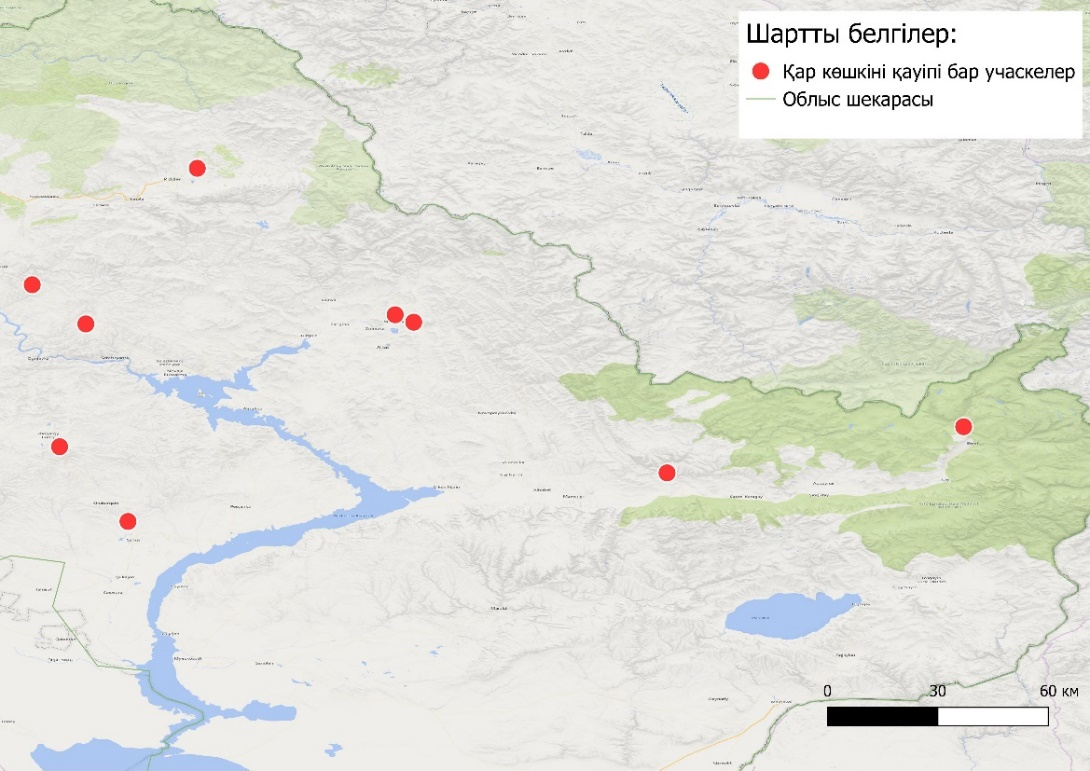
\includegraphics[width=0.7\textwidth]{media/ict2/image199}
	\caption*{1 - сурет. Шығыс Қазақстанда көшкін қауіпі бар аймақтардың орналасуы}
\end{figure}

\begin{multicols}{2}
{\bfseries Материалдар мен әдістер.} Табиғи апаттардың тәуекелдерін
бағалау, жер бедерінің ерекшеліктерін ескере отырып, көшкін қауіпі бар
учаскелерін зерттеу стратегиясын әзірлеу және инфрақұрылымын жоспарлау
үшін геоморфологиялық карталар негізінде жергілікті жердің
геоморфологиялық талдау жүргізілді. Геоморфологиялық карталар - бұл жер
беті бедерінің нысандарын көрсететін мамандандырылған тақырыптық
карталар {[}11, 12{]}.

Көшкіндерді зерттеу едәуір дәрежеде геоморфологиялық карталарға
сүйенеді. Олар көшкін қауіптілігін талдауға және болжауға, сондай-ақ
аумақтық қорғау шараларын әзірлеуге көмектеседі. Мұндай карталарда
көшкін қауіпі бар аудандарды анықтауға және көшкін процестерінің
динамикасын түсінуге мүмкіндік беретін ақпарат бар.

Тақырыптық карталар жер бедерінің цифрлық моделі негізінде жасалынды.
Google Earth Pro-ның координаталық және биіктік деректері негізінде
зерттелетін учаскелердің биіктік карталары мен 3D модельдері жасалды.
Google Earth Pro биіктік деректерін әртүрлі көздерден, соның ішінде SRTM
(Shuttle Radar Topography Mission) деректерінен алады. Цифрлық
модельдерді құру негізі ретінде SRTM деректері таңдап алынды. SRTM -
радиолокациялық қашықтықтан зондтау деректерін пайдалана отырып, Жер
бедерінің дәлдігі жоғары цифрлық моделін жасауға бағытталған халықаралық
жоба болып табылады. Бұл жобаның барысында жер бетінің басым бөлігі
(80\% жуық) үшін жер бедердің жаһандық цифрлық модельдерін жасауға
мүмкіндік беретін деректер жиналды {[}13, 14{]}.

Қазіргі заманғы әдістермен жасалатын дәлдігі жоғары цифрлық модель
негізінде геоморфологиялық талдау (аэрофототүсіріс, LiDAR, жерүстілік
лазерлік сканерлеу).

Түсіріс DJI Matrice 300 RTK және лидар Emesent Hovermap ST ұшқышсыз
авиациялық жүйесінің (сурет 2) көмегімен жүргізілді. Шығыс Қазақстан
облысының аумағында таңдалған көшкін жинағыштардың сандық 3D моделін
түсіру және жасау келесі ретпен орындалады (сурет 3).
\end{multicols}

\begin{figure}[H]
	\centering
	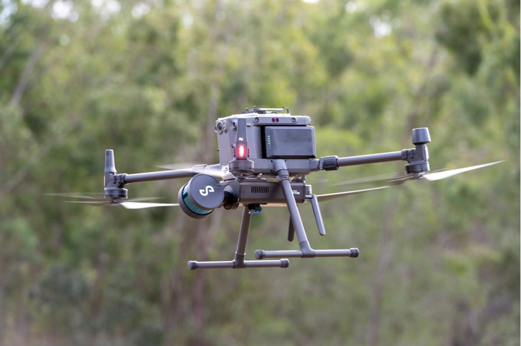
\includegraphics[width=0.7\textwidth]{media/ict2/image200}
	\caption*{2 - сурет. Hovermap лидарымен DJI Matrice 300 RTK ҰҰА көрінісі}
\end{figure}

\begin{figure}[H]
	\centering
	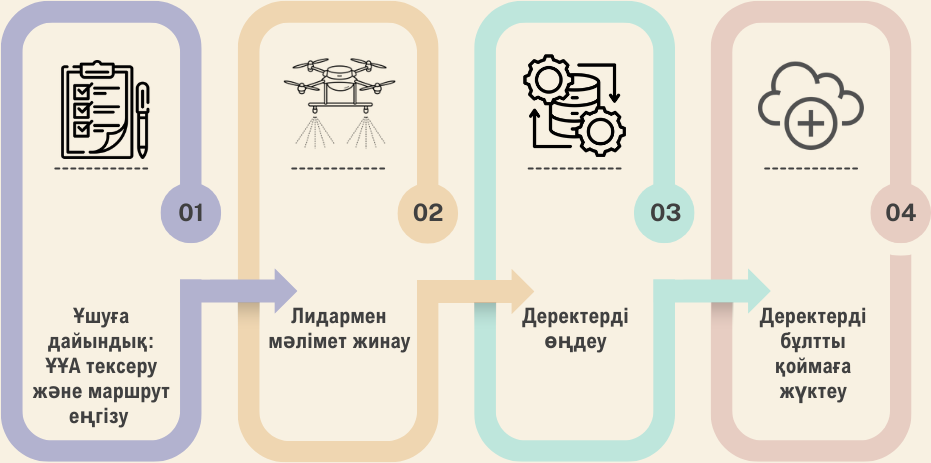
\includegraphics[width=0.7\textwidth]{media/ict2/image201}
	\caption*{3 - сурет. ҰҰА және LiDAR көмегімен зерттеуді жүргізу реті}
\end{figure}

\begin{multicols}{2}
Зерттеу объектісі ретінде Шығыс Қазақстан облысында көшкін қауіпі бар
аймақтар алынған. Далалық жұмыстар «Зубовская» тауы, Проходная өзені,
Лайлы өзені, Таинты өзені, Богатыревская копь аймақтарында жүргізілді.

{\bfseries Нәтижелер мен талқылау.} Лидар технологиясы аумақ пен нысандар
туралы жоғары дәлдіктегі үш өлшемді ақпаратты алуға мүмкіндік береді
және оның негізінде жасалған цифрлық модельдер картографияда, құрылыста,
инженерлік нысандарды жобалауда, геологияда, межелеуде және қалалық
ортада кеңінен қолданылады. Лидарлық түсіріс материалдары бойынша
цифрлық модельдерді құру әртүрлі қызмет салаларында сұранысқа ие,
аумақтар мен объектілердің дәл және интерактивті үш өлшемді көріністерін
алуға мүмкіндік беретін мамандандырылған технологиялық және аналитикалық
процестер сериясын қамтиды {[}15{]}.

Лидардан алынған деректерді бастапқы өңдеу Aura бағдарламасында жүзеге
асырылады (сурет 4). Бағдарлама лидардан бұлтты нүктелерді құруға
арналған. Бағдарламада шығу деректерімен күрделі емес операцияларды
жүргізуге болады. Нүктелерді кесу, сирету, координаталық жүйені ауыстыру
және т.б. Сондай-ақ шығу деректерін әртүрлі жазықтықта көруге болады
(сурет 5).
\end{multicols}

\begin{figure}[H]
	\centering
	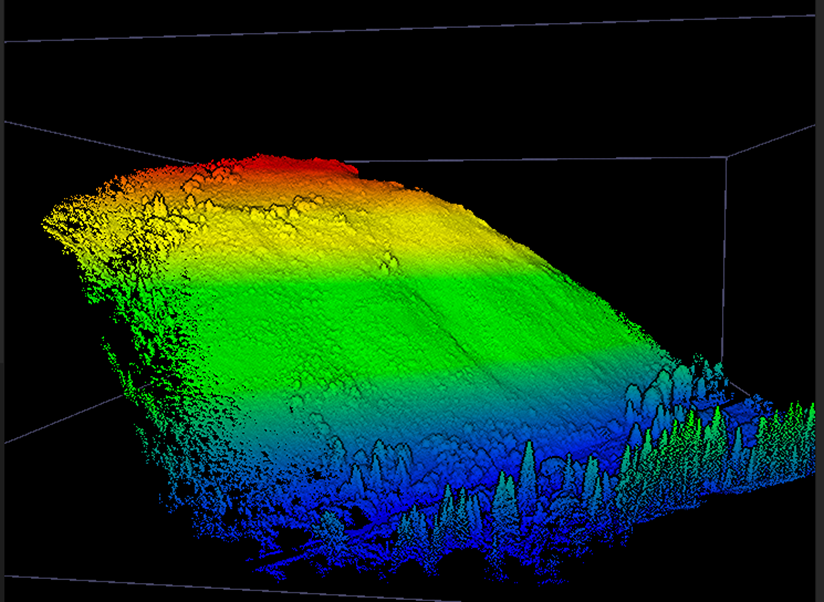
\includegraphics[width=0.7\textwidth]{media/ict2/image202}
	\caption*{4 - сурет. Aura бағдарламасындағы түсіріс нәтижелері}
\end{figure}

\begin{figure}[H]
    \centering
    \begin{subfigure}[t]{0.45\textwidth}
        \centering
        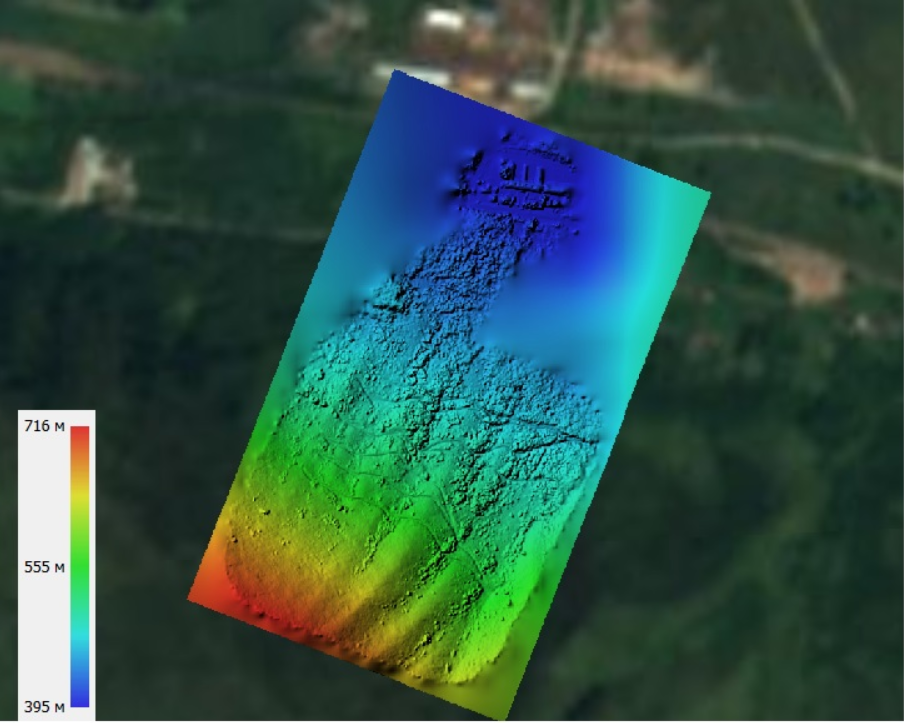
\includegraphics[width=\textwidth]{media/ict2/image203}
        \caption*{а)}
    \end{subfigure}
    \begin{subfigure}[t]{0.45\textwidth}
        \centering
        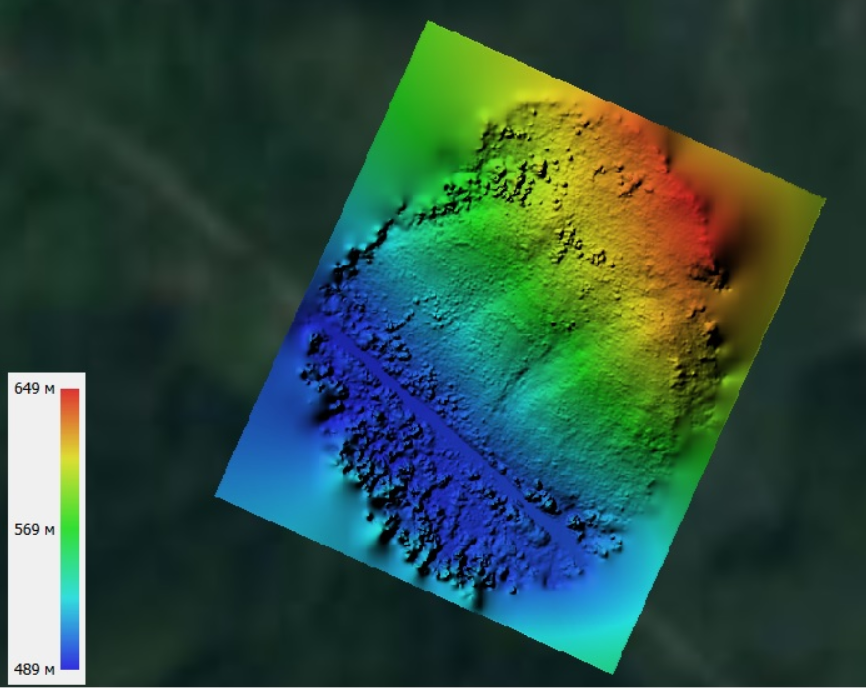
\includegraphics[width=\textwidth]{media/ict2/image204}
        \caption*{ә)}
    \end{subfigure}
\end{figure}
\begin{figure}[H]
    \centering
    \begin{subfigure}[t]{0.45\textwidth}
        \centering
        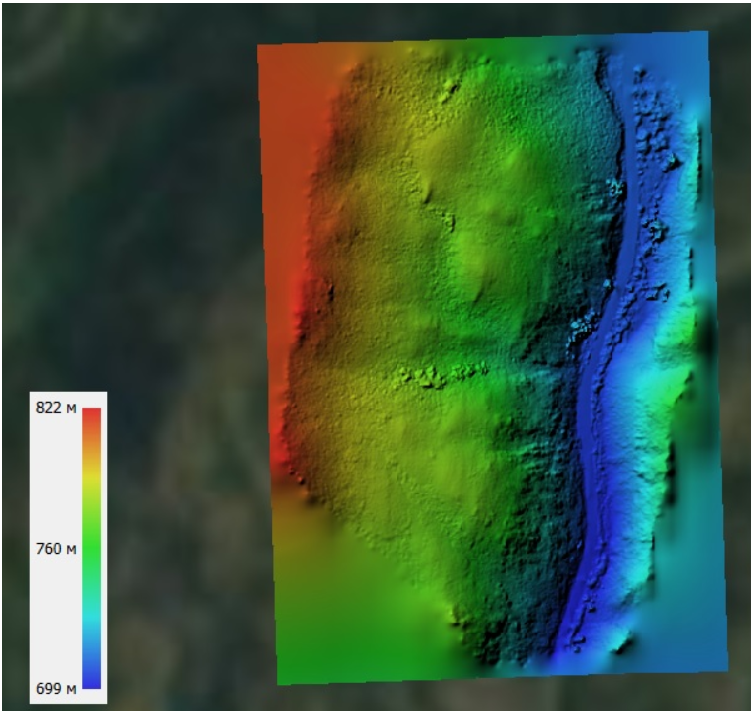
\includegraphics[width=\textwidth]{media/ict2/image205}
        \caption*{б)}
    \end{subfigure}
    \begin{subfigure}[t]{0.45\textwidth}
        \centering
        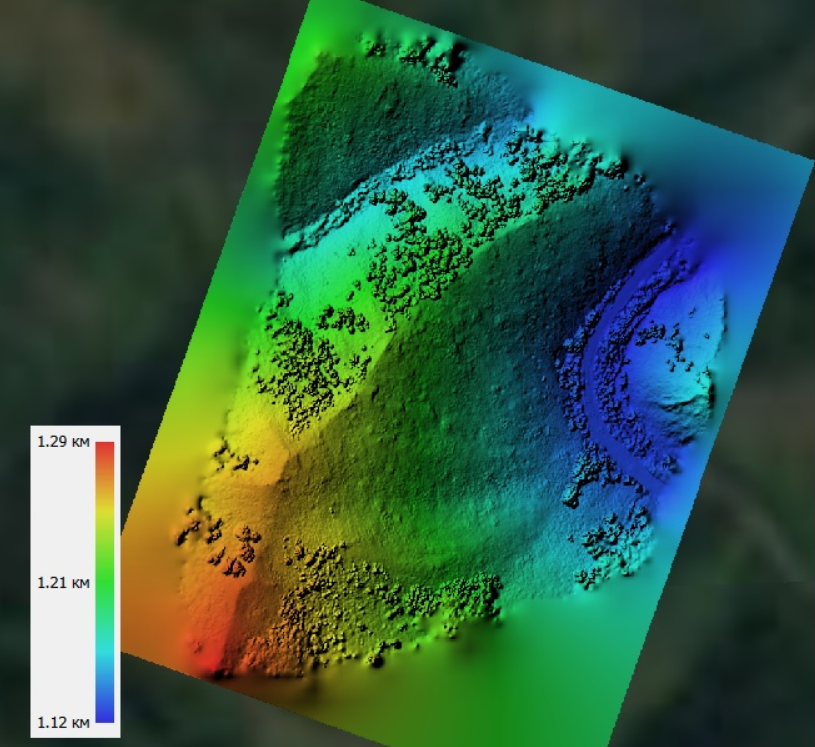
\includegraphics[width=\textwidth]{media/ict2/image206}
        \caption*{в)}
    \end{subfigure}
    \begin{subfigure}[t]{0.7\textwidth}
        \centering
        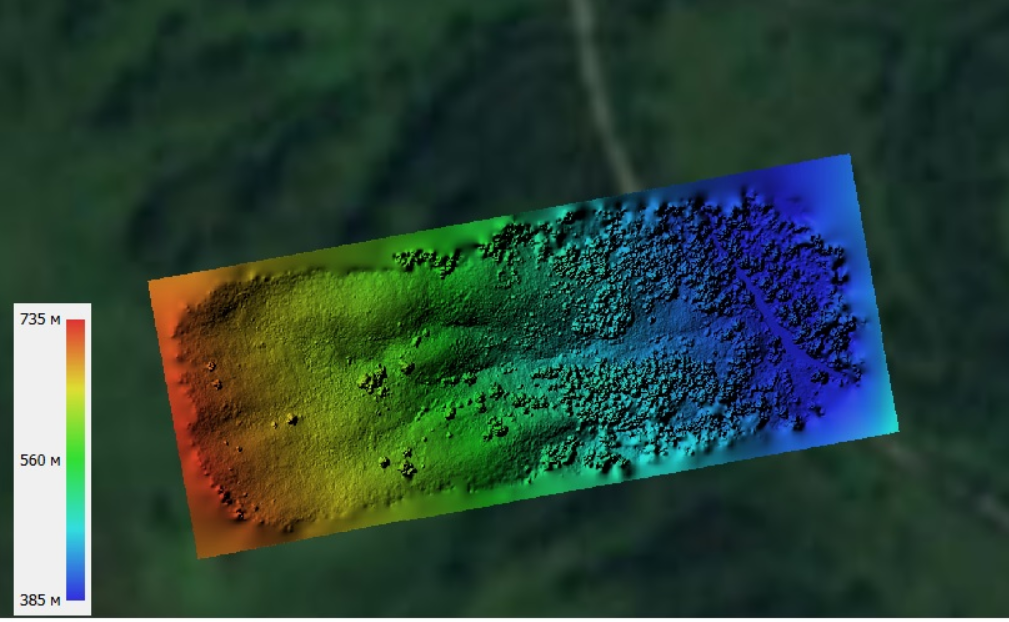
\includegraphics[width=\textwidth]{media/ict2/image207}
        \caption*{г)}
    \end{subfigure}
    \caption*{5 - сурет. Лидардан алынған өңдеу деректері: а) «Зубовская» тауы; ә) Проходная өзені; б) Лайлы өзені; в) Таинты өзені; г) Богатыревская копь}
\end{figure}

\begin{multicols}{2}
Зерттеу жүргізу барысында лидар түсіру технологиясының дәстүрлі түсіру
әдістерімен салыстырғанда бірқатар маңызды артықшылықтарға ие, сонымен
қатар кемшіліктерін де атап өтуге болады (1-кесте).

Сондықтан лидар түсірісі кеңістіктік деректерді жинаудың жылдам, дәл
және жоғары сапалы әдісі болып табылады, бұл әр түрлі мәселелерді шешу
үшін ақпараттың егжей-тегжейін, алу жылдамдығын, сенімділігі мен
дәлдігін едәуір арттыра алады {[}16{]}.

SRTM мәліметтері негізінде цифрлық модельдерді құру.

Биіктік карталар QGIS 3.36 нұсқасындағы бағдарламалық жасақтамада SRTM
негізінде жасалынды. Жүктелген растрлар Topography сызықтық градиенті
бар бір арналы жалған түсті кескінге түрлендірілді. Цифрлық деректер
(биіктік белгілері) жергілікті жердің биіктігіне сәйкес тең
диапазондарға бөлінген.

\end{multicols}

\begin{longtblr}[
  caption = {\bfseries 1 - кесте. Лидарлық түсірістің артықшылықтары мен кемшіліктері},
  label = none,
  entry = none,
]{
  width = \linewidth,
  colspec = {Q[475]Q[469]},
  row{1} = {c},
  hlines,
  vlines,
}
\textbf{Артықшылықтары} & \textbf{Кемшіліктер}\\
Кеңістіктің
			жоғары дәлдігі мен нақтылығы (сантиметр
			мен миллиметрге дейін), бұл микро жер
			бедерін жақсы анықтауға және жергілікті
			геоморфологиялық процестерді зерделеуге
			мүмкіндік береді. & Деректерді
			алуға және оларды өңдеуге жұмсалатын
			жоғары құн мен еңбек шығындары.\\
Үдерістердің
			мониторингі және жер бедерінің
			динамикасы жағдайында бақылауларды
			үнемі жаңарту және толықтыру мүмкіндігі. & Үлкен
			аумақтарда өлшеуді жүзеге асыру қиын.\\
Өсімдіктер
			мен құрылыс салынған аумақтардың аз
			әсері (әсіресе орман алқаптары мен
			жерге дәл енуді қамтамасыз ететін
			LiDAR үшін). & Деректерді
			жинау жүйесінде технологиялық
			шектеулердің болуы (мысалы, ауа райы
			жағдайлары, дрондарды пайдалануға
			шектеулер, өңдеу үшін күрделі аппаратура
			мен мамандардың қажеттілігі).\\
Әдістеменің
			үлкен әмбебаптығы мен икемділігі:
			түрлі тапсырмаларға түсіру параметрлерін
			өзгерту мүмкіндігі. & {~\\~}
\end{longtblr}

\begin{multicols}{2}
Сондай-ақ, картаға қар өлшейтін рейкалар, көшкін қауіпі бар учаскелердің
шекаралары, цифрлық модельдер деректері негізінде құрылған автомобиль
жолдары және т.б. түріндегі картографиялық жағдайлар қосылды.

Морфометриялық мәлеметтерді талдау нәтижесінде көшкін қауіпі бар
учаскелердің жердің биіктігі бойынша сипаттама берілген {[}17{]}.

«Зубовская» тауының учаскесі 480 - 800 м деңгейінде орналасқан (сурет
6). № 1 - 5 көшкін жинағыштар 480 - 560 м биіктікте орналасқан, көшкін
жинағыштардың абсолюттік белгілері оңтүстік-шығыста жоғары орналасқан.
Ең үлкен көшкін жинағы (№ 10) 800 м биіктікте орналасқан (сурет 7).
\end{multicols}

\begin{figure}[H]
	\centering
	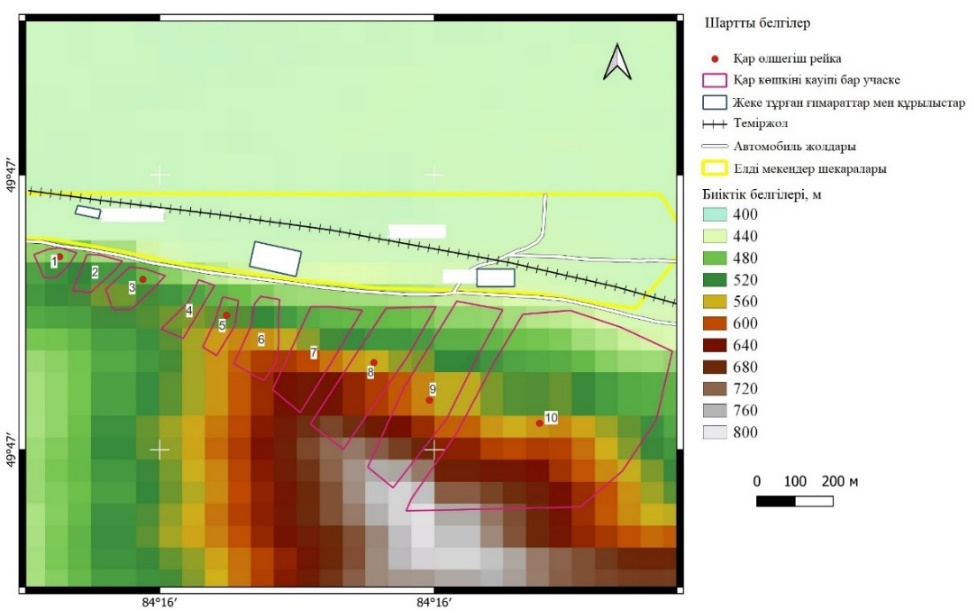
\includegraphics[width=0.65\textwidth]{media/ict2/image208}
	\caption*{6 - сурет. «Зубовск» тауы учаскесінің биіктік картасы (SRTM мәліметтері негізінде)}
\end{figure}

\begin{figure}[H]
	\centering
	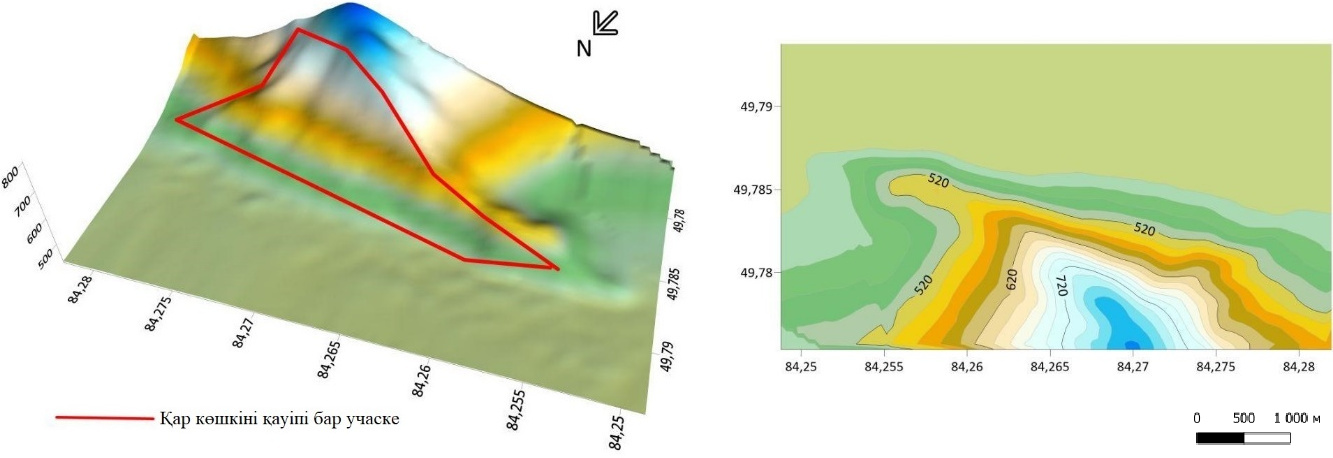
\includegraphics[width=0.8\textwidth]{media/ict2/image210}
	\caption*{7 - сурет. Google Earth Pro деректері негізінде биіктік карталары мен 3D модельдері («Зубовск» тауы учаскесі)}
\end{figure}

\begin{multicols}{2}
Проходная өзенінің учаскесінде, Горная Ульбинка ауылында (сурет 8)
көшкін жинағыштар негізінен (№ 22 дейін) 460 - 580 м биіктікте
орналасқан, оңтүстік-шығысқа қарай, көшкін жинағыштар биіктігінің таулар
арасындағы арақашықтықта (№ 23 - 26) 850 - 880 м дейін жетеді (сурет 9).
\end{multicols}

\begin{figure}[H]
	\centering
	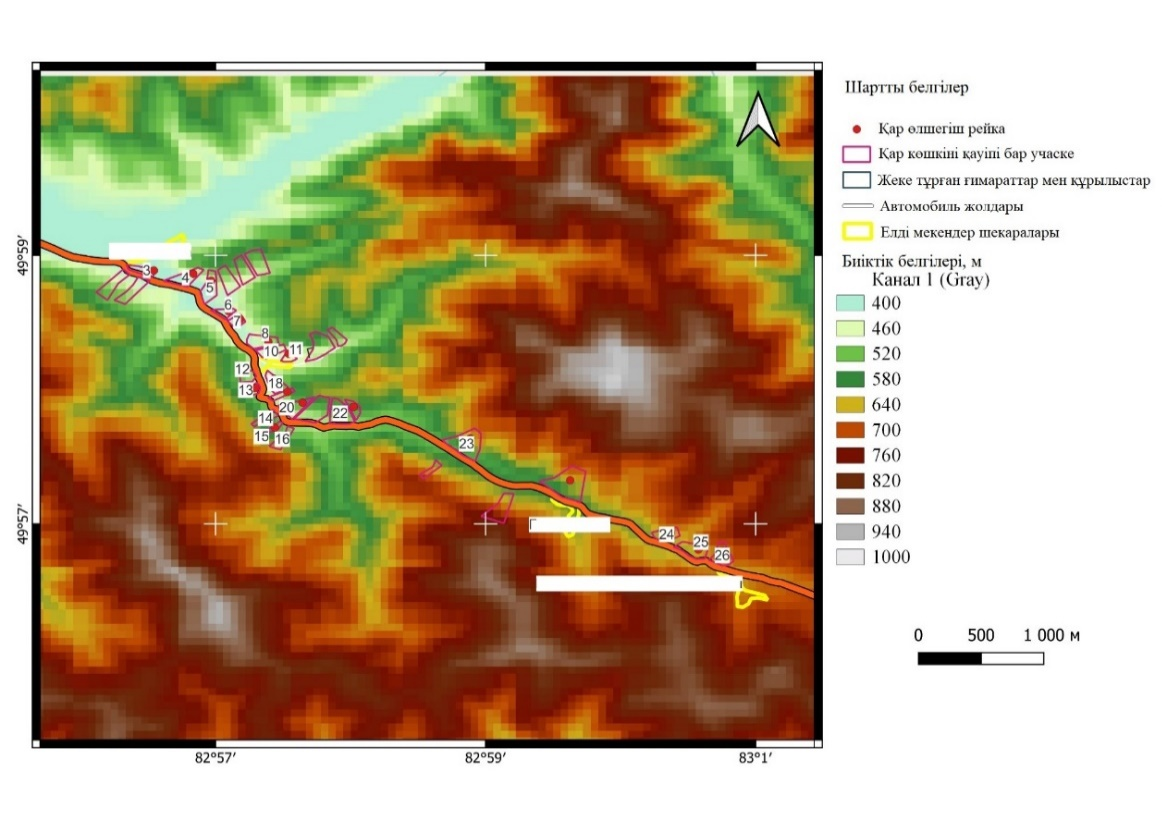
\includegraphics[width=0.6\textwidth]{media/ict2/image211}
	\caption*{8 - сурет. Проходная өзені учаскесінің биіктік картасы (SRTM мәліметтері негізінде)}
\end{figure}

\begin{figure}[H]
	\centering
	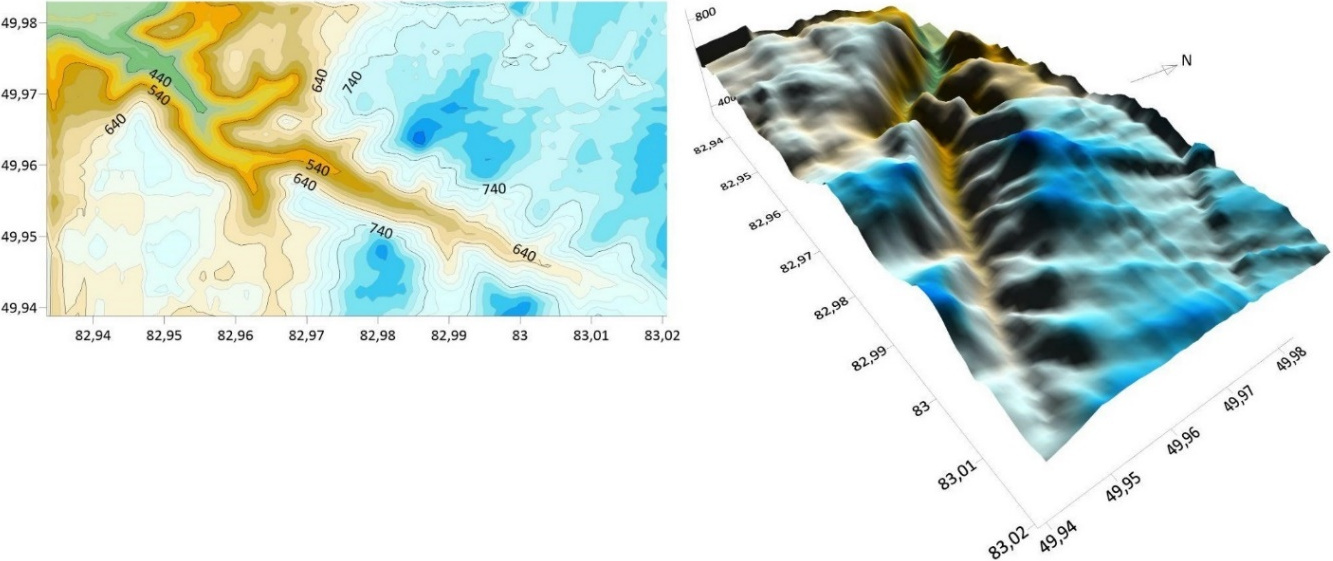
\includegraphics[width=0.7\textwidth]{media/ict2/image212}
	\caption*{9 - сурет. Google Earth Pro деректері негізінде биіктік карталары мен 3D модельдері (Проходная өзені учаскесі)}
\end{figure}

\begin{multicols}{2}
Лайлы өзені учаскесінің барлық 3 қар көшкін жинағыштары (сурет 10)
өзеннің оң жағалауында 750 - 850 м биіктікте орналасқан (сурет 11),
Тайынты өзені ауданы бойынша көршілес учаске (сурет 12) Тайынты өзенінің
оң жағалауындағы тар шатқалда орналасқан. № 1 - 10 қар көшкін
жинағыштардың 950 - 1200 м диапазонында асболюттік белгілері бар, № 11,
12 қар көшкін жинағыштар тік баурайларда орналасқан. № 12 көшкін
жинағыштың жоғарғы бөлігінің биіктігі 1450 м тең (сурет 13).
\end{multicols}

\begin{figure}[H]
	\centering
	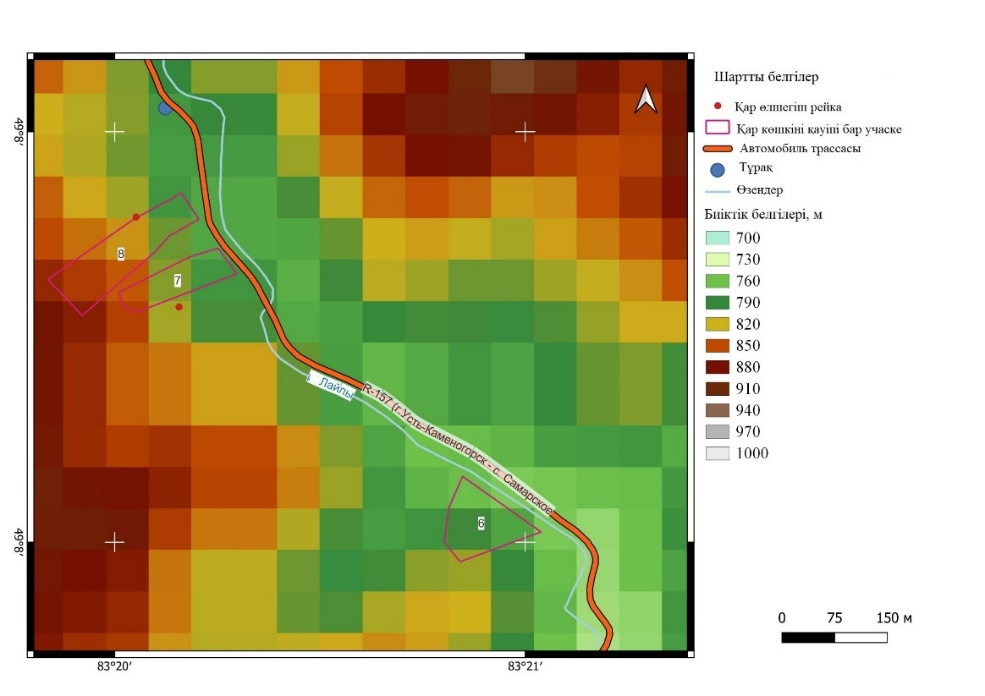
\includegraphics[width=0.8\textwidth]{media/ict2/image213}
	\caption*{10 - сурет. Лайлы өзені учаскесінің биіктік картасы (SRTM мәліметтері негізінде)}
\end{figure}

\begin{figure}[H]
	\centering
	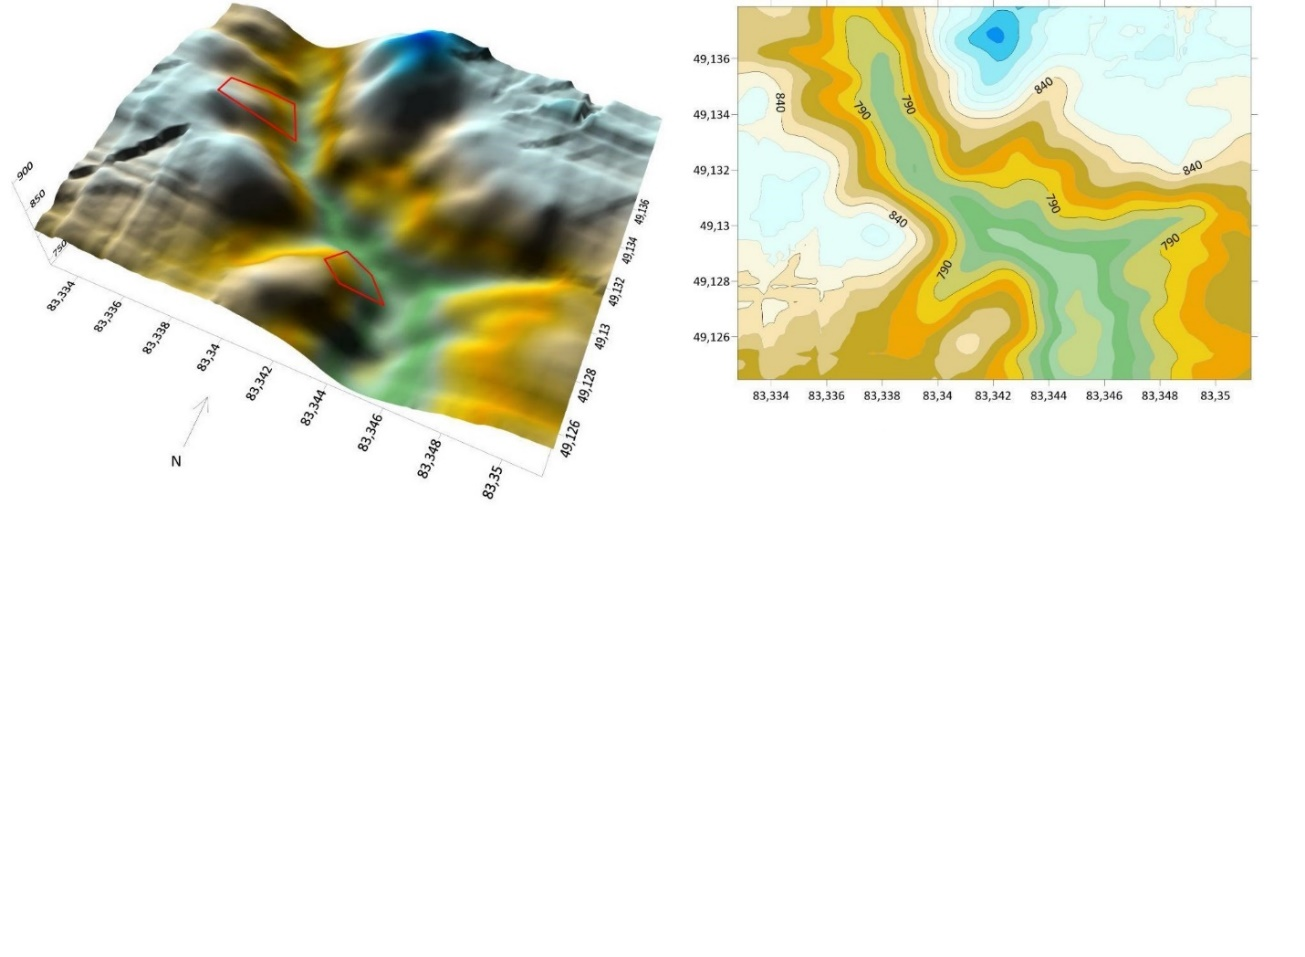
\includegraphics[width=0.9\textwidth]{media/ict2/image214}
	\caption*{11 - сурет. Google Earth Pro деректері негізінде биіктік карталары мен 3D модельдері (Лайлы өзені учаскесі)}
\end{figure}

\begin{figure}[H]
	\centering
	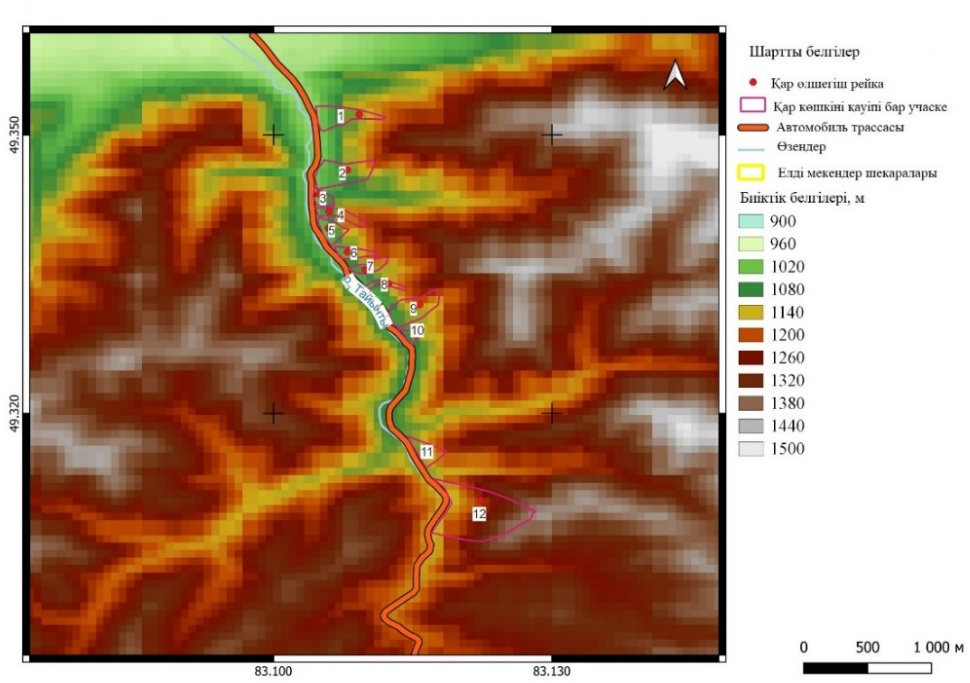
\includegraphics[width=0.8\textwidth]{media/ict2/image215}
	\caption*{12 - сурет. Таинты өзені учаскесінің биіктік картасы (SRTM мәліметтері негізінде)}
\end{figure}

\begin{figure}[H]
	\centering
	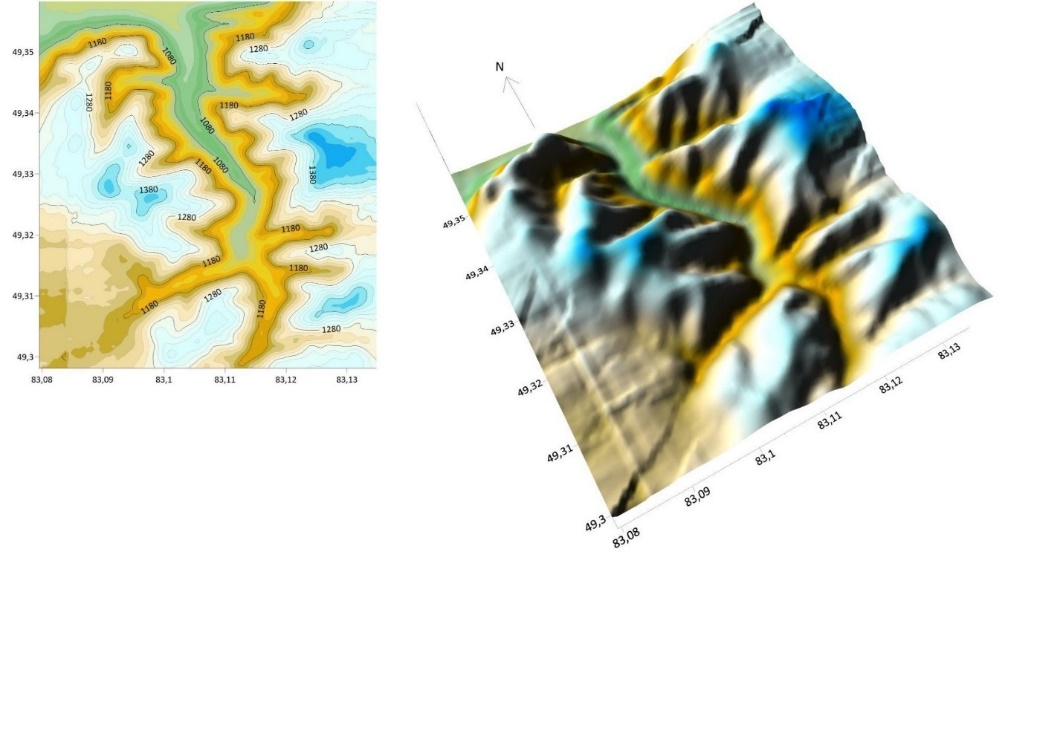
\includegraphics[width=0.9\textwidth]{media/ict2/image216}
	\caption*{13 - сурет. Google Earth Pro деректері негізінде биіктік карталары мен 3D модельдері (Таинты өзенінің учаскесі)}
\end{figure}

«Богатыревская копь» учаскесінің көшкін жинағыштары (сурет 14) жотаның
солтүстік-шығыс беткейлерінде орналасқан, ол автожолдан кейін қиялы өзен
алқабына өтеді. Абсолюттік белгілер 480-800 м шегінде өзгереді (сурет
15).

\begin{figure}[H]
	\centering
	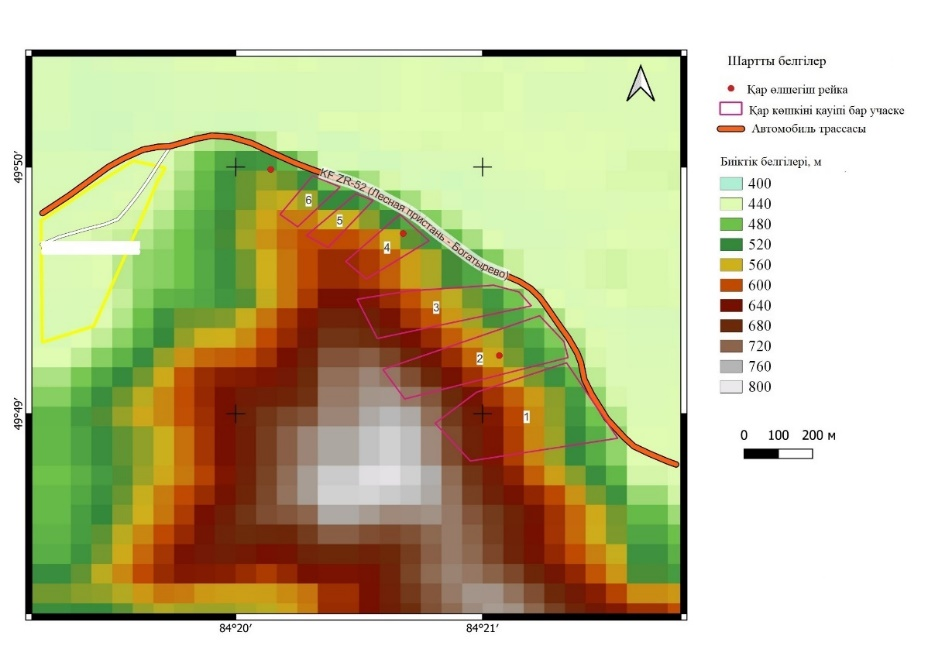
\includegraphics[width=0.8\textwidth]{media/ict2/image217}
	\caption*{14 - сурет. Богатыревская копь учаскесінің биіктігінің картасы (SRTM мәліметтері негізінде)}
\end{figure}

\begin{figure}[H]
	\centering
	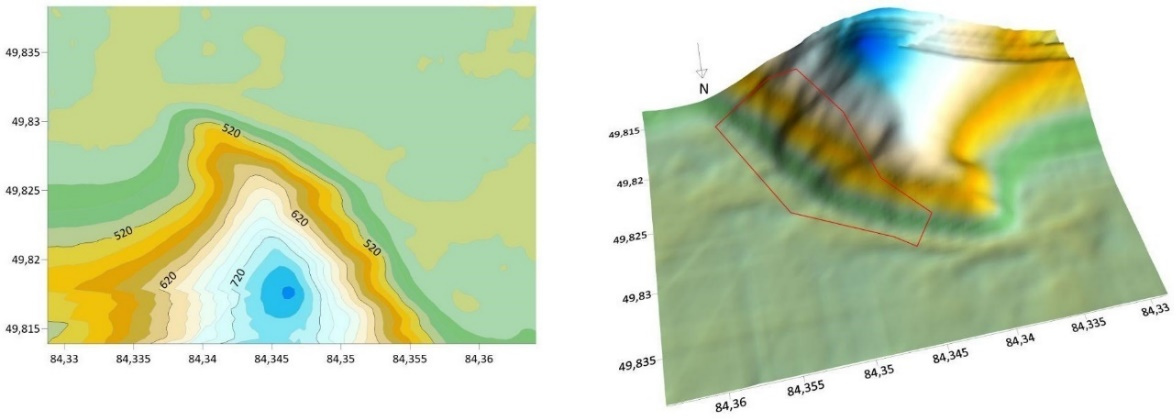
\includegraphics[width=0.9\textwidth]{media/ict2/image218}
	\caption*{15 - сурет. Google Earth Pro деректері негізінде биіктік карталары мен 3D модельдері (Богатыревская копь учаскесі)}
\end{figure}

Нақты учаскелер мен аумақтар үшін түсіру жұмыстары және кейіннен әуедегі
немесе жердегі фотосуреттерді өңдеу негізінде (фотограмметриялық немесе
лазерлік технологияларды қолдана отырып) цифрлық модельдер жасау жолымен
жеке жүргізіледі.

Цифрлық модельдерді құру негізі ретінде SRTM мәліметтерін қолдану
нәтижесінде олардың келесі артықшылықтары мен кемшіліктерін көрсетуге
болады (2-кесте).

\begin{longtblr}[
  caption = {\bfseries 2 - кесте. Цифрлық модель құру негізі ретінде SRTM мәліметтерін қолданудың артықшылықтары мен кемшіліктері},
  label = none,
  entry = none,
]{
  width = \linewidth,
  colspec = {Q[425]Q[517]},
  row{1} = {c},
  hlines,
  vlines,
}
\textbf{Артықшылықтары} & \textbf{Кемшіліктер}\\
Қолжетімділік:
			деректер тегін және қоғамдық пайдалануға
			ашық. & Көлеңкеден,
			өсімдіктермен жабудан, құрылыстардан
			және т.б. кейбiр қателiктер мен
			артефактiлердiң болуы.\\
Жақсы
			жаһандық жабын: қолайлы рұқсатпен жер
			бетін қамту (шамамен 30 м және 90 м, бұрын
			90 м пайдаланылған, енді көбінесе 30 м
			жақсартылған деректер ұсынылады). & Кеңістіктік
			шешімі жоғары емес (әдетте 30 - 90 м). Бұл
			жер бедерiнiң шағын ауқымды ерекшелiктерiн
			зерделеу кезiнде егжей-тегжейлi
			жергiлiктi процестердi зерттеу талаптарын
			әрдайым қанағаттандырмайды.\\
Деректерді
			жаһандық геоморфологиялық зерттеулерде
			пайдалануға мүмкіндік беретін
			бірізділігі. & Тік
			өлшеулердің салыстырмалы төмен дәлдігі
			(орташа ± 3 - 5 м), әсіресе өсімдіктермен
			жабылған немесе құрылыс салынған
			аудандарда, ұсақ ауқымды талдаудың
			нашарлаған дәлдігі.\\
Жұмыстың
			ыңғайлылығы мен қарапайымдылығы,
			форматтардың таралуы. & SRTM
			бір мезгілде алынғандықтан (2000 жыл),
			зерттеушілердің өздері деректерді
			жаңартуға немесе нақтылауға болмайды.
\end{longtblr}

\begin{multicols}{2}
Тік беткейлердің картасын жасау үшін SRTM деректері пайдаланылды. Құрал
ретінде QGIS морфометриялық талдау плагині қолданылды. Морфометриялық
есептеулерден кейін растр бір арналы жалған түсті бейнеге ауыстырылды.
``Turbo'' градиенті бірдей градус интервалдарымен қолданылды {[}18,
19{]}. Нәтижесінде участкелер бойынша морфометриялық карталар құрылды
(сурет 16).
\end{multicols}

\begin{figure}[H]
    \centering
    \begin{subfigure}[t]{0.42\textwidth}
        \centering
        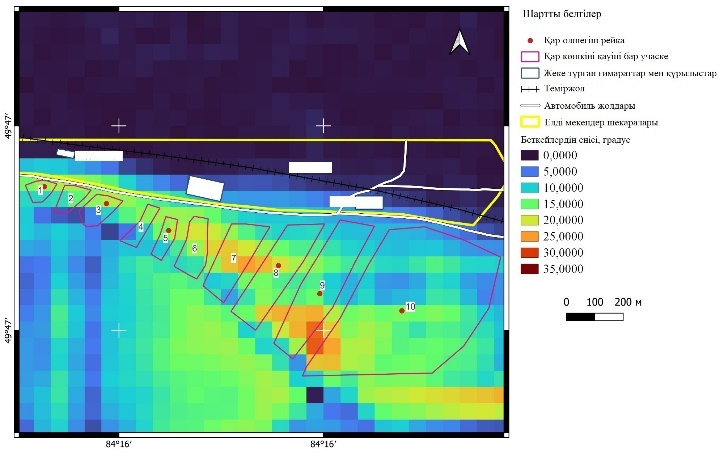
\includegraphics[width=\textwidth]{media/ict2/image219}
        \caption*{а)}
    \end{subfigure}
    \begin{subfigure}[t]{0.42\textwidth}
        \centering
        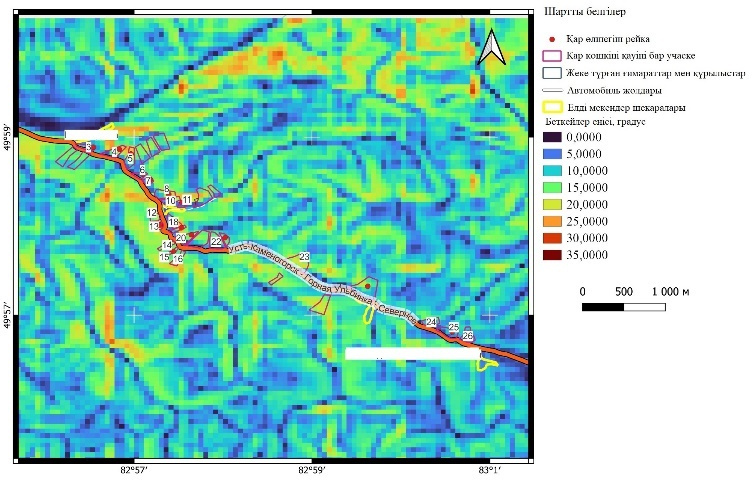
\includegraphics[width=\textwidth]{media/ict2/image220}
        \caption*{ә)}
    \end{subfigure}
    \\
    \begin{subfigure}[t]{0.42\textwidth}
        \centering
        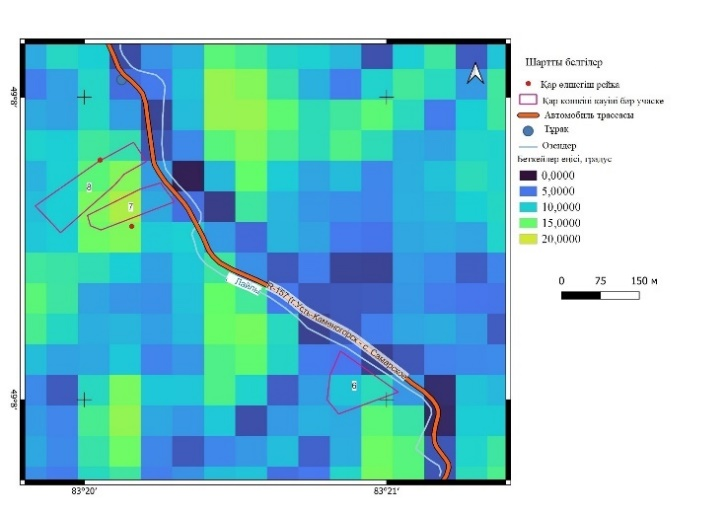
\includegraphics[width=\textwidth]{media/ict2/image221}
        \caption*{б)}
    \end{subfigure}
    \begin{subfigure}[t]{0.42\textwidth}
        \centering
        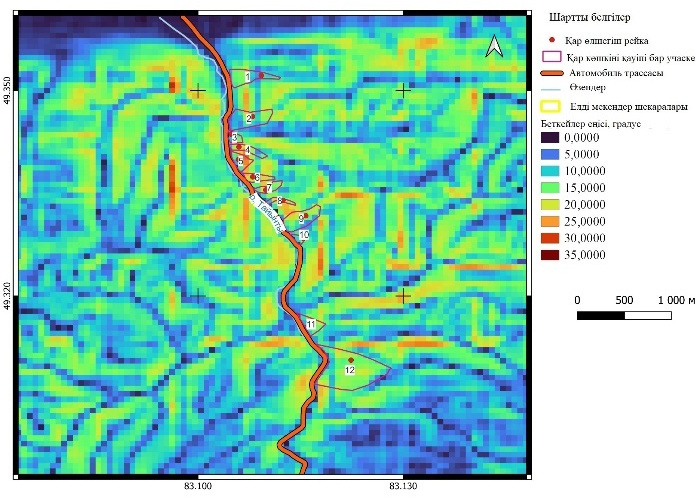
\includegraphics[width=\textwidth]{media/ict2/image222}
        \caption*{в)}
    \end{subfigure}
\end{figure}
\begin{figure}[H]
    \centering
    \begin{subfigure}[t]{0.42\textwidth}
        \centering
        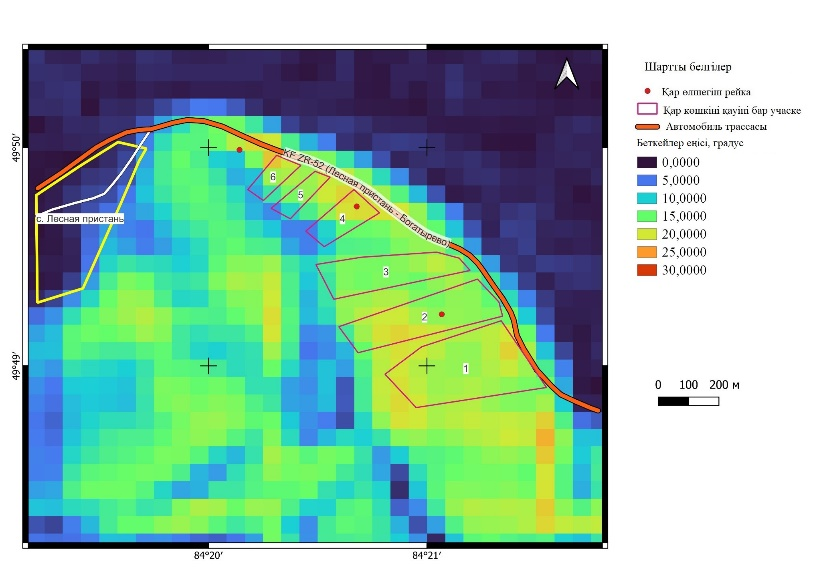
\includegraphics[width=\textwidth]{media/ict2/image223}
        \caption*{г)}
    \end{subfigure}
    \caption*{{\bfseries 16 - сурет. Морфометриялық карта: а) «Зубовск» тауы; ә) Проходная өзені; б) Лайлы өзені; в) Таинты өзені; г) Богатыревская копь}}
\end{figure}

Лидар түсірілімдері мен биіктік карталарының нәтижелерін талдау
негізінде қар көшкінінің түсуіне неғұрлым бейім көлбеу бұрыштары бар
учаскелер анықталды (3-кесте).

\begin{longtblr}[
  caption = {\bfseries 3 - кесте. Көшкін қауіпі бар учаскелердің беткейлері еңісінің ең жоғары және ең төменгі мәндері},
  label = none,
  entry = none,
]{
  cells = {c},
  hlines,
  vlines,
}
\textbf{Учаскенің			атауы} & \textbf{Еңістердің			ең аз мәні,			º} & \textbf{Еңістердің			ең көп			мәні,			º}\\
«Зубовск»
			тауы & 10 & 30\\
Проходная
			өзені & 15 & 30\\
Лайлы
			өзені & 5 & 20\\
Таинты
			өзені & 15 & 30\\
Богатыревская
			копь & 15 & 25
\end{longtblr}

\begin{multicols}{2}
{\bfseries Қорытынды.} SRTM деректерін аймақтық талдау және зерттеудің
алдын-ала кезеңі, аумақты жалпы зерттеу, жер бедерінің негізгі
ерекшеліктерін іздеу үшін пайдалу дұрыс.

Жоғары дәлдіктегі цифрлық модельдер жергілікті және нақты процестерді
егжей-тегжейлі талдау және бақылау үшін, шағын аумақтарды инженерлік,
экологиялық және ғылыми зерттеулерде немесе жоғары нақталығы мен дәлдік
қажет жерлерде оңтайлы.

Екі әдістің де артықшылықтары бар және жалпы ауқымды талдаудан (SRTM)
негізгі жер бедері учаскелерін (жоғары дәлдіктегі цифрлық модельдер)
егжей-тегжейлі зерттеуге көшу мүмкіндіктерінің арқасында бір-бірін сәтті
толықтыра алады. Белгілі бір тәсілді немесе осы тәсілдердің жиынтығын
таңдау толығымен аумақтық міндеттерге және геоморфологиялық
зерттеулердің ауқымына байланысты.

Алынған морфометриялық карталар мен оларды талдау негізінде көшкін қаупі
бар учаскелер тік беткейлерде орналасқанын атап өткен жөн, учаскелер
негiзiнен 25-45º тiк диапазондағы баурайларда орналасқан. Көшкін
жинағыштардың көпшілігі 15-25º құламалы баурайларда орналасқан.

Бұл мәліметтер ары қарай ШҚО бойынша қар көшкіні қауіпі бар учаскелерді
бақылау жүргізуге және қар көшкінің болжау бойынша геоақпараттық
бағдарламаларды жобалауға қолданылады.

Бұл зерттеу 2023-2025 жылдарға арналған BR21882022 «Мониторинг жүйелерін
әзірлеу және оларды орналастырудың ғылыми негіздемесі үшін Шығыс
Қазақстан облысындағы көшкін белсенділігін зерттеу» БНҚ бағдарламасы
шеңберінде жүргізілді.
\end{multicols}

\begin{center}
{\bfseries Әдебиеттер}
\end{center}

\begin{references}
1. Rakhymberdina, M., Levin, E., Daumova, G., Bekishev Y., Assylkhanova,
Z., Kapasov, A. Combined Remote Sensing and GIS Methods for Detecting
Avalanches in Eastern Kazakhstan // ES Energy and Environment. - 2024. -
Vol.26. - P.1350. DOI 10.30919/esee1350.

2. Aydin A., Eker R. GIS-based snow avalanche hazard mapping:
bayburt-aşağı dere catchment case // Journal of Environmental Biology.-
2017. -Vol.38(5).- P.937-943. DOI 10.22438/jeb/38/5(si)/gm-10.

3. Wastl M., Stötter J., Kleindienst H., Avalanche risk assessment for
mountain roads: a case

study from Iceland// Natural Hazards. - 2011. - Vol.56(2). DOI
10.1007/s11069-010-9703-64.

4. Bühler Y., Bebi P., Christen M., Margreth S., Stoffel L., Stoffel A.,
Marty C., Schmucki G., Caviezel A., Kühne R., Wohlwend S., Bartelt P.
Automated avalanche hazard indication mapping on a statewide scale //
Natural Hazards and Earth System Sciences. - 2022. - Vol.22 (6) - P.
1825-1843. DOI 10.5194/nhess-22-1825-2022.

5. Kurt T. Avalanche Hazards with Mitigation in Turkey and Qualitative
Risk Assessment for Snow \\Avalanches in Ayder (Rize, NE Turkey) Using
Combination of GIS, Remote Sensing Techniques and Field Studies. In
Applications of Space Techniques on the Natural Hazards in the MENA
Region // Springer International Publishing: New York, NY, USA. - 2022.
- P.533--567. DOI
\href{http://dx.doi.org/10.1007/978-3-030-88874-9_23}{10.1007/978-3-030-88874-9\_23}.

6. Aydın A., Eker R., Odabaşı Y.B. Generating avalanche hazard
indication map and determining snow avalanche protection forests in
çaykara-Trabzon (NE-Turkey) // Forestist. - 2022. - Vol.72 (1). - P.
62-72. DOI 10.5152/forestist.2021.20060.

7. Eckerstorfer M., Christiansen H.H. Meteorology, Topography and
Snowpack Conditions Causing Two Extreme Mid-Winter Slush and Wet Slab
Avalanche Periods in High Arctic Maritime Svalbard //\\
\href{https://www.researchgate.net/journal/Permafrost-and-Periglacial-Processes-1099-1530?_tp=eyJjb250ZXh0Ijp7ImZpcnN0UGFnZSI6InB1YmxpY2F0aW9uIiwicGFnZSI6InB1YmxpY2F0aW9uIn19}{Permafrost
and Periglacial Processes}.- 2012.- Vol.23. - P.15-25. DOI
\href{http://dx.doi.org/10.1002/ppp.734}{10.1002/ppp.734}.

8. Denissova N., Nurakynov S., Petrova O., Chepashev D., Daumova G.,
Yelisseyeva A. Remote sensing techniques for assessing snow avalanche
formation factors and building hazard monitoring systems // Atmosphere.
- 2024. - Vol.15(11). - P.1343. DOI 10.3390/atmos15111343.

9. Omirzhanova Zh.T., Urazaliev A.S., Aimenov A.T. GIS for predicting
the avalanche zones in the mountain regions of Kazakhstan //
\href{https://www.researchgate.net/journal/The-International-Archives-of-the-Photogrammetry-Remote-Sensing-and-Spatial-Information-Sciences-2194-9034?_tp=eyJjb250ZXh0Ijp7ImZpcnN0UGFnZSI6InB1YmxpY2F0aW9uIiwicGFnZSI6InB1YmxpY2F0aW9uIn19}{The
International Archives of the Photogrammetry Remote Sensing and Spatial
Information Sciences}.- 2015. - XL-2/W4. - P.39--44. DOI
10.5194/isprsarchives-XL-2-W4-39-2015.

10. Rakhymberdina M., Bekishev Y., Denissova N., Daumova, G.,
Assylkhanova, Z. Investigation Of Avalanche-Prone Areas of East
Kazakhstan Based on Space Imagery Materials // In Proceedings of the 9th
International Conference on Cartography and GIS, Nessebar, Bulgaria. --
2024. ISSN 1314-0604

11. Николаева С.А., Савчук Д.А., Кузнецов А.С. Особенности датирования
селей, лавин и камнепадов в верховьях р. Актру (Северо-Чуйский хребет,
Центральный Алтай) по травмам деревьев //Геоэкология. Инженерная
геология, гидрогеология, геокриология - 2017. - № 4. -- С.31-43.

12. Кюль Е.В. Оценка изменения ландшафтов лавинной деятельностью (по
ландшафтным признакам частоты схода лавин) //Известия
Кабардино-Балкарского научного центра РАН. -2014. - № 3. - С.53-59.

13. Yang L., Meng X., Zhang X. SRTM DEM and its applications advanced
//International Journal of Remote Sensing 2011. - Vol.32 (14). - P.
3875-3896.
DOI\href{http://dx.doi.org/10.1080/01431161003786016}{10.1080/01431161003786016}.

14. Rodriguez E., Morris C.S., Belz J.E. A global assessment of the
SRTM~performance //Photogrammetric Engineering \& Remote Sensing. -
2006. -Vol.72. - P.249-260. DOI 10.14358/PERS.72.3.249.

15. Eitel J.U.H., Hö, B., Vierling L.A., Abellán A., Asner G.P., Deems
J.S., Glennie C.L., Joerg P.C., Lewinter A.L., Magney T.S., Mandlburger
G., Morton D.C., Müller J., Vierling K.T. Beyond 3-D: The new spectrum
of lidar applications for earth and ecological sciences //
\href{https://asu.elsevierpure.com/en/publications/beyond-3-d-the-new-spectrum-of-lidar-applications-for-earth-and-e}{\hfill\break
Remote Sensing of Environment}.-2016.-Vol.186.-P.372--392. DOI
10.1016/j.rse.2016.08.018

16. Chong Z.J., Qin B., Bandyopadhyay T., Ang M., Frazzoli E., Rus D.
Synthetic 2D LIDAR for precise vehicle localization in 3D urban
environment // In Proceedings of the IEEE International Conference on\\
Robotics and Automation (ICRA), Karlsruhe, Germany. - 2013. - P.
1554--1559. DOI \\10.1109/ICRA.2013.6630777.

17. Maggioni M., Gruber U. The influence of topographic parameters on
avalanche release dimension and frequency // Cold Regions Science and
Technology. - 2003.-Vol.37 (3). - P.407-419. DOI
10.1016/S0165-232X(03)00080-6.

18. Крючков А.Н., Абламейко С.В., Апарин Г.П., Соболь Л.Н. Методы
оперативного анализа состояния местности на основе моделей цифровых карт
и аэро-космоснимков // Штучний інтелект. - 2010. - № 3. - С.329-340.

19. Singh D.K., Mishra V.D., Gusain H.S. Simulation and analysis of a
snow avalanche accident in Lower Western Himalaya // India, Journal of
the Indian Society of Remote Sensing. -- 2020. -- Vol.48 (11). - P.
1555-1565. DOI 10.1007/s12524-020-01178-5.
\end{references}

\begin{center}
{\bfseries References}
\end{center}

\begin{references}
1. Rakhymberdina, M., Levin, E., Daumova, G., Bekishev Y., Assylkhanova,
Z., Kapasov, A. Combined Remote Sensing and GIS Methods for Detecting
Avalanches in Eastern Kazakhstan // ES Energy and Environment. - 2024. -
Vol.26. - P.1350. DOI 10.30919/esee1350.

2. Aydin A., Eker R. GIS-based snow avalanche hazard mapping:
bayburt-aşağı dere catchment case // Journal of Environmental Biology.-
2017. -Vol.38(5).- P.937-943. DOI 10.22438/jeb/38/5(si)/gm-10.

3. Wastl M., Stötter J., Kleindienst H., Avalanche risk assessment for
mountain roads: a case

study from Iceland// Natural Hazards. - 2011. - Vol.56(2). DOI
10.1007/s11069-010-9703-64.

4. Bühler Y., Bebi P., Christen M., Margreth S., Stoffel L., Stoffel A.,
Marty C., Schmucki G., Caviezel A., Kühne R., Wohlwend S., Bartelt P.
Automated avalanche hazard indication mapping on a statewide scale //
Natural Hazards and Earth System Sciences. - 2022. - Vol.22 (6) - P.
1825-1843. DOI 10.5194/nhess-22-1825-2022.

5. Kurt T. Avalanche Hazards with Mitigation in Turkey and Qualitative
Risk Assessment for Snow \\Avalanches in Ayder (Rize, NE Turkey) Using
Combination of GIS, Remote Sensing Techniques and Field Studies. In
Applications of Space Techniques on the Natural Hazards in the MENA
Region // Springer International Publishing: New York, NY, USA. - 2022.
- P.533--567. DOI
\href{http://dx.doi.org/10.1007/978-3-030-88874-9_23}{10.1007/978-3-030-88874-9\_23}.

6. Aydın A., Eker R., Odabaşı Y.B. Generating avalanche hazard
indication map and determining snow avalanche protection forests in
çaykara-Trabzon (NE-Turkey) // Forestist. - 2022. - Vol.72 (1). - P.
62-72. DOI 10.5152/forestist.2021.20060.

7. Eckerstorfer M., Christiansen H.H. Meteorology, Topography and
Snowpack Conditions Causing Two Extreme Mid-Winter Slush and Wet Slab
Avalanche Periods in High Arctic Maritime Svalbard //\\
\href{https://www.researchgate.net/journal/Permafrost-and-Periglacial-Processes-1099-1530?_tp=eyJjb250ZXh0Ijp7ImZpcnN0UGFnZSI6InB1YmxpY2F0aW9uIiwicGFnZSI6InB1YmxpY2F0aW9uIn19}{Permafrost
and Periglacial Processes}.- 2012.- Vol.23. - P.15-25. DOI
\href{http://dx.doi.org/10.1002/ppp.734}{10.1002/ppp.734}.

8. Denissova N., Nurakynov S., Petrova O., Chepashev D., Daumova G.,
Yelisseyeva A. Remote sensing techniques for assessing snow avalanche
formation factors and building hazard monitoring systems // Atmosphere.
- 2024. - Vol.15(11). - P.1343. DOI 10.3390/atmos15111343.

9. Omirzhanova Zh.T., Urazaliev A.S., Aimenov A.T. GIS for predicting
the avalanche zones in the mountain regions of Kazakhstan //
\href{https://www.researchgate.net/journal/The-International-Archives-of-the-Photogrammetry-Remote-Sensing-and-Spatial-Information-Sciences-2194-9034?_tp=eyJjb250ZXh0Ijp7ImZpcnN0UGFnZSI6InB1YmxpY2F0aW9uIiwicGFnZSI6InB1YmxpY2F0aW9uIn19}{The
International Archives of the Photogrammetry Remote Sensing and Spatial
Information Sciences}.- 2015. - XL-2/W4. - P.39--44. DOI
10.5194/isprsarchives-XL-2-W4-39-2015.

10. Rakhymberdina M., Bekishev Y., Denissova N., Daumova, G.,
Assylkhanova, Z. Investigation Of Avalanche-Prone Areas of East
Kazakhstan Based on Space Imagery Materials // In Proceedings of the 9th
International Conference on Cartography and GIS, Nessebar, Bulgaria. --
2024. ISSN 1314-0604

11. Nikolaeva S.A., Savchuk D.A., Kuznecov A.S. Osobennosti datirovanija
selej, lavin i kamnepadov v verhov' jah r. Aktru
(Severo-Chujskij hrebet, Central' nyj Altaj) po travmam
derev' ev //Geojekologija. Inzhenernaja geologija,
gidrogeologija, geokriologija - 2017. - № 4. -- S.31-43.{[}in
Russian{]}

12. Kjul'{} E.V. Ocenka izmenenija landshaftov lavinnoj
dejatel' nost' ju (po landshaftnym
priznakam chastoty shoda lavin) //Izvestija Kabardino-Balkarskogo
nauchnogo centra RAN. -2014. - № 3. - S.53-59. {[}in Russian{]}

13. Yang L., Meng X., Zhang X. SRTM DEM and its applications advanced
//International Journal of Remote Sensing 2011. - Vol.32 (14). - P.
3875-3896.
DOI\href{http://dx.doi.org/10.1080/01431161003786016}{10.1080/01431161003786016}.

14. Rodriguez E., Morris C.S., Belz J.E. A global assessment of the
SRTM~performance //Photogrammetric Engineering \& Remote Sensing. -
2006. -Vol.72. - P.249-260. DOI 10.14358/PERS.72.3.249.

15. Eitel J.U.H., Hö, B., Vierling L.A., Abellán A., Asner G.P., Deems
J.S., Glennie C.L., Joerg P.C., Lewinter A.L., Magney T.S., Mandlburger
G., Morton D.C., Müller J., Vierling K.T. Beyond 3-D: The new spectrum
of lidar applications for earth and ecological sciences //
\href{https://asu.elsevierpure.com/en/publications/beyond-3-d-the-new-spectrum-of-lidar-applications-for-earth-and-e}{\hfill\break
Remote Sensing of Environment}.-2016.-Vol.186.-P.372--392. DOI
10.1016/j.rse.2016.08.018

16. Chong Z.J., Qin B., Bandyopadhyay T., Ang M., Frazzoli E., Rus D.
Synthetic 2D LIDAR for precise vehicle localization in 3D urban
environment // In Proceedings of the IEEE International Conference on
Robotics and Automation (ICRA), Karlsruhe, Germany. - 2013. - P.
1554--1559. DOI \\10.1109/ICRA.2013.6630777.

17. Maggioni M., Gruber U. The influence of topographic parameters on
avalanche release dimension and frequency // Cold Regions Science and
Technology. - 2003.-Vol.37 (3). - P.407-419. DOI
10.1016/S0165-232X(03)00080-6.

18. Krjuchkov A.N., Ablameĭko S.V., Aparin G.P., Sobol'{}
L.N. Metody operativnogo analiza sostojanija mestnosti na osnove modeleĭ
cifrovyh kart i ajero-kosmosnimkov // Shtuchnij іntelekt. - 2010. - № 3.
- S.329-340. {[}in Russian{]}

19. Singh D.K., Mishra V.D., Gusain H.S. Simulation and analysis of a
snow avalanche accident in Lower Western Himalaya // India, Journal of
the Indian Society of Remote Sensing. -- 2020. -- Vol.48 (11). - P.
1555-1565. DOI 10.1007/s12524-020-01178-5.
\end{references}

\begin{authorinfo}
\emph{{\bfseries Авторлар туралы мәліметтер}}

Капасов А. К. - Жер туралы ғылымдар мектебі оқытушы, Д. Серікбаев
атындағы ШҚТУ" КЕАҚ, Қазақстан, ШҚО, Өскемен қаласы, e-mail:
AKapasov@edu.ektu.kz;

Денисова Н.Ф. - Физика-математика ғылымдарының кандидаты, Цифрлық
офицер, Д. Серікбаев атындағы ШҚТУ" КЕАҚ, Өскемен, Қазақстан, e-mail:
NDenisova@ektu.kz;

Рахымбердина. М.Е. - PhD докторы, Жер туралы ғылымдар мектебі, деканы,
Д. Серікбаев атындағы ШҚТУ" КЕАҚ, Өскемен, Қазақстан, e-mail:
MRahymberdina@edu.ektu.kz;

Сапарходжаев Н.П. - PhD докторы, қауымдастырылған профессор, басқарма
төрағасы-ректор, Рудный индустриялық институты, Рудный Қазақстан, e-mail:
nursp81@gmail.com;

Бекишев Е.Т. - Жер туралы ғылымдар мектебі оқытушы, Д. Серікбаев
атындағы ШҚТУ" КЕАҚ, Өскемен, Қазақстан, e-mail:
YBekishev@edu.ektu.kz;

\emph{{\bfseries Information about the authors}}

Kapasov A.K. - Lecturer School of Earth Sciences, NAO "D. Serikbaev
EKTU", Ust-Kamenogorsk, Kazakhstan,
e-mail: \\AKapasov@edu.ektu.kz;

Denisova N.F. - Candidate of Physico-mathematical Sciences, Digital
Officer, NAO "D. Serikbaev EKTU", Ust-Kamenogorsk, Kazakhstan, e-mail:
NDenisova@ektu.kz;

Rahymberdina M.Е. - doctor PhD, Dean School of Science of the Earth ,
NAO "D. Serikbaev EKTU", Ust-Kamenogorsk, Kazakhstan,  e-mail:
MRahymberdina@edu.ektu.kz;

Saparhodzhaev N.P. - PhD, Associate Professor, Chairman of the
Board-Rector, Rudny industrial university, Rudny, Kazakhstan, e-mail:
nursp81@gmail.com;

Bekishev Е.Т. -Lecturer School of Earth Sciences, NAO "D. Serikbaev
EKTU", Ust-Kamenogorsk, Kazakhstan, e-mail: \\YBekishev@edu.ektu.kz;
\end{authorinfo}
